\chapter{Expérimentation}
\label{chap:exp}

\section{Introduction}
Dans ce chapitre nous parlons des logiciels, matériels et des données que nous utilisons pour implémenter et tester notre algorithme. Ensuite, nous présentons le résultat de notre algorithme sur ces données. Nous conclurons aussi notre travail à la fin de ce chapitre.

\section{Logiciels et matériels}
Dans ce stage, nous avons utilisé des logiciels et des matériels listées ci-dessous :\\
Logiciels
\begin{itemize}
\item Extraction des caractéristiques : SIFT[low99], K-Means(pour clustering)
\item Méthode pour la classification : SGD binaire (implémentation Pegasos), LibSVM(pour la comparaison)
\item En C/C++, sous GNU-Linux
\end{itemize}
Matériels
\begin{itemize}
\item PC core-i7, 8 cœurs, 3G RAM
\item Système d'exploitation : GNU-Linux Fedora 20
\end{itemize}
Nos propositions
\begin{itemize}
\item Classification multi-classes: MC-SGD et MC-SGD parallèle, implémentés en C/C++ en utilisant l'OpenMP
\item Outils pour étudier notre algorithme: MC-SGD-Toy, basé sur SVM-Toy\cite{cl01}
\end{itemize}

\section{Jeux de données}
Les données sont traitées à partir des bases d'images en utilisant la méthode SIFT avec le nombre de dimension et le modèle BoVW avec le nombre de mots visuels dans la colonne 4 et 5 dans la table ci-dessous.

\begin{table}[H]
\begin{center}
    \begin{tabular}{ | c | c | c | c | c |}
    \hline
    Données & \#classes & \#exemples & \#dimension(SIFT) & \#mots(BoVW) \\ \hline

    Cal 101 & 101 & 1515 & 128 & 124000 \\ \hline

    Cal 7 3D & 7 & 4290 & 128 & 5000 \\ \hline 

    ImgNet 3d & 10 & 4450 & 128 & 5000 \\ \hline

    ImgNet & 10 & 4450 & 128 & 50000 \\ \hline

    \end{tabular}
\end{center}
\caption{Information sur des données}
\label{tab:infod1}
\end{table}


\section{Méthode SGD binaire}
Pour cette étape, nous voulons comparer le SGD binaire avec la LibSVM pour voir si quelle méthode est plus efficace. Nous utilisons ci-dessous la base de données binaire (2 classes) de la LibSVM \cite{svmdata1}, Adult avec la taille d'exemple d'entrées différente.\\

Dans cette expérimentation, les données sont linéaires. C'est la raison pour laquelle nous avons utilisé le SVM linéaire car elle est plus efficace que les autres fonctions de noyau. Pour l'algorithme SGD binaire, nous avons utilisé $T = 10000$ itérations et dans chaque itération nous choisissons 10 exemples aléatoires. Avec le SGD, le résultat change un peu (moins de 10\%) chaque cas de test car cet algorithme choisit aléatoirement des exemples dans chaque itération, donc, nous avons testé 10 fois chaque exemple et fait la moyenne pour comparer avec le résultat de la bibliothèque LibSVM.

\begin{table}
\begin{center}
    \begin{tabular}{ | c | c | c | c | c | c | c |}
    \hline
    Données & \#Exemple & LIBSVM(\%) & SGD(\%) & LIBSVM(s) & SGD(s) & $\frac{SVM(s)}{SGD(s)}$ \\ \hline
    
    a1a & 1,605 & 83.82 & 84.30 & 0.438 & 0.044 & 10 \\ \hline
    
    a2a & 2,265 & 84.27 & 84.48 & 0.826 & 0.045 & 18 \\ \hline
    
    a3a & 3,185 & 84.33 & 84.31 & 6.990 & 0.050 & 139 \\ \hline
    
    a4a & 4,781 & 84.44 & 84.33 & 3.162 & 0.043 & 73 \\ \hline
    
    a5a & 6,414 & 84.39 & 84.33 & 5.766 & 0.048 & 120 \\ \hline
    
    a6a & 11,220 & 84.72 & 84.34 & 20.846 & 0.049 & 425 \\ \hline
    
    a7a & 16,100 & 84.83 & 84.45 & 42.392 & 0.056 & 757 \\ \hline
    
    a8a & 22,696 & 85.16 & 84.95 & 91.500 & 0.054 & 1,694 \\ \hline
    
    a9a & 32,561 & 84.97 & 84.64 & 299.648 & 0.064 & 4,682 \\ \hline
    
    \end{tabular}
\end{center}
\caption{Comparaison entre LIBSVM et SGD-SVM}
\label{tab:svmsgd}
\end{table}

\begin{figure}[ht!]
\centering
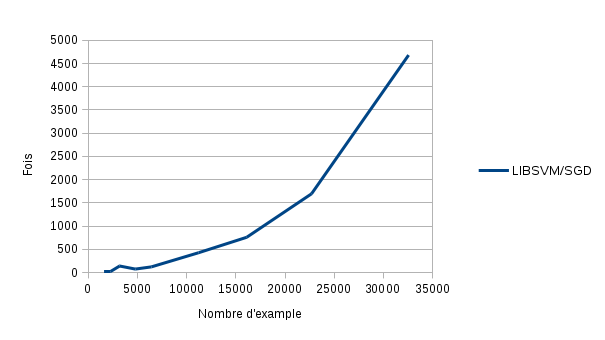
\includegraphics[width=150mm]{images/res}
\caption{Comparaison de la vitesse entre LibSVM et SGD binaire}
\label{fig:res}
\end{figure}

\pagebreak
Par rapport au table \ref{tab:svmsgd}, nous trouvons que le taux de classification du SGD et de la LibSVM est presque pareil tandis que le temps d'apprendre est différent. La vitesse du SGD est très vite que la vitesse de la LibSVM. Cet avantage du SGD est plus clair quand le nombre d'exemples d'apprentissage augmente. Cette chiffre est démontrée dans la colonne 7 de table \ref{tab:svmsgd} ou aussi dans le figure \ref{fig:res}.\\

Les données que nous avons utilisé ont 123 caractéristiques. Nous trouvons que quand le nombre d'exemple est de 1,605, l'algorithme SGD est plus vitesse que la LibSVM de 10 fois, mais quand le nombre d'exemple de 32,561, le SGD plus vitesse que la LibSVM 4,682 fois. Ce chiffre confirme que le SGD est beaucoup plus vitesse que la LibSVM, surtout pour les grandes données. Donc, l'algorithme SGD s'adapte mieux au problème de classification d'image dont la base de données est très grande. En raison de son avantage, nous voulons le développer pour qu'elle puisse résoudre le problème de classification multi-classes afin d'utiliser dans le domaine de classification d'images.

\section{MC-SGD pour la classification multi-classes}
\begin{itemize}
\item Protein : 3 classes, 17000 exemples, 357 caractéristiques
\item Mnist : 10 classes, 60000 exemples, 780 caractéristiques
\item SVM : function linéaire
\item SGD : -iter 500 -k 100 -lambda 0.05
\end{itemize}

\begin{table}[h]
\begin{center}
    \begin{tabular}{ | c | c | c | c | c | c | c | c |}
    \hline
    Données & SVM(\%) & 1-vs-all(\%) & 1-vs-1(\%) & SVM(s) & 1-vs-all(s) & 1-vs-1(s) & $\frac{SVM(s)}{SGD(s)}$ \\ \hline
    
    Protein & 68.23 & 68.41 & 69.10 & 551 & 0.20 & 0.19 & \textbf{2755} \\ \hline
    
    Mnist & 86.92 & 86.46 & 89.71 & 2810 & 0.72 & 4.23 & \textbf{3902.8} \\ \hline
    
    \end{tabular}
\end{center}
\caption{Comparaison entre LIBSVM et MC-SGD parallèle}
\label{tab:pmcsvm}
\end{table}

En générale, le résultat de classification du MC-SGD ne meilleure pas quand on compare avec la LibSVM. Par contre, le temps d'apprendre est beaucoup plus vite que la LibSVM pour le problème de classification multi-classes. La table \ref{tab:pmcsvm} est une preuve.
Pour le MC-SGD, nous trouvons que le résultat de classification de la version one-vs-one est un peu mieux que la version one-vs-all. Le temps  d'apprentissage de deux options est presque pareil pour le problème de 3 classes. Par contre, pour le problème de 10 classes, la version one-vs-one est plus lent que la version one-vs-all 5.8 fois. Ce chiffre va augmenter très vite quand le nombre de classes augmente. Pendant ce stage, nous nous concentrons à développer un algorithme qui peut améliorer le temps du SVM, donc, nous trouvons que la version one-vs-all est un bon choix. Pour les tests suivants, nous ne faisons que la comparaison entre la version one-vs-all du MC-SGD avec la LibSVM.

\section{MC-SGD pour la classification d'images}
Comme nous avons parlé dans le processus, notre processus pour la classification d'images comprend 3 étapes principales : extraction des descripteurs avec le descripteur SIFT, construit le dictionnaire avec la méthode K-moyenne et l'apprentissage automatique pour la classification avec la méthode MC-SGD. Dans la partie précédente nous avons présenté le résultat de l'algorithme MC-SGD (l'étape 3, l'étape d'apprentissage automatique) avec la base de données existante. Maintenant, nous appliquons la méthode Sac de Mots pour préparer les entrées pour l'algorithme MC-SGD avec les bases d'images pour voir si la méthode MC-SGD s'adapte pour le problème de classification d'images.
\begin{itemize}
\item SVM : function linéaire
\item SGD : -iter 1000 -k 10 -lambda 0.6
\end{itemize}

\begin{table}[h]
\begin{center}
    \begin{tabular}{ | c | c | c | c | c | c |}
    \hline
    Données & SVM(\%) & SGD(\%) & SVM(s) & SGD(s) & $\frac{SVM(s)}{SGD(s)}$ \\ \hline

    Cal 101 & 61.52 & 65.12 & 2873 & 106.95 & \textbf{26.9} \\ \hline
    
    Cal 7 3D & 91.52 & 88.3 & 113.4 & 0.81 & \textbf{140} \\ \hline 

    ImgNet 3d & 76.54 & 75.8 & 144 & 0.90 & \textbf{160} \\ \hline
    
    ImgNet & 84.08 & 86.58 & 327 & 1.64 & \textbf{199.4} \\ \hline
    
    \end{tabular}
\end{center}
\caption{Comparaison entre LIBSVM et MC-SGD parallèle pour la classification d'images}
\label{tab:pimgclasssvm}
\end{table}

Le tableau \ref{tab:pimgclasssvm} montre que le pourcentage de classification de la LibSVM est presque égale au MC-SGD. Par contre, la LibSVM est plus lent que le MC-SGD de 26 à 199 fois. Nous rappelons que la LibSVM utilise l'option one-vs-one et le MC-SGD utilise l'option one-vs-all. Donc, si la base d'image augmente plus de catégories (le nombre de classes), l'algorithme MC-SGD sera plus vitesse si l'on compare avec l'algorithme de la LibSVM.

%\pagebreak
Pour être facile de faire la comparaison sur la vitesse entre notre algorithme et la LibSVM, nous vous montrons la graphique \ref{fig:res1} (le taux de SVM/MC-SGD)
\begin{figure}[H]
\centering
\includegraphics[width=150mm]{images/res1}
\caption{Comparaison de SVM et MC-SGD (SVM/MC-SGD)}
\label{fig:res1}
\end{figure}

Non seulement plus vite que le SVM quand le nombre de classes augmente, mais aussi sur le nombre d'exemple d'apprentissage. La graphique ci-dessus peut montrer ce que nous expliquons. Le taux de temps de SVM/MC-SGD augmente selon le nombre d'exemple très claire dans cette graphique. Précisément, quand le nombre d'exemple de 1515, ce taux est de 26.9 mais ce taux est de 199.4 quand le nombre d'exemple est de 60000. La raisons est que notre algorithme n'a pas besoin de prendre tous les exemples pour l'apprentissage.\\
